Solving the blocks introduced in the previous sections need 2 different approaches. The graphs of the maps can be split in 2 groups. The first one, considers problems where there are no loops and at most one node with more than 2 legs Examples include:
$ \vcenter{\hbox{ \pepob{3}{2}{{"1","1","1","1"}}{{"1","1","1","1"}}{{0,0,0,1,0,1}} }} \text{and} \vcenter{\hbox{  \mpob{4}{ {,"1","2","1",}  }{}{}{}{{,,,,,}} }}$ (see \cref{subsec:lin_block_Def}).
These will be reduced to a standard matrix problem, and solve with matrix (pseudo-) inversion. The other group, of course, constitutes the nonlinear problems. This includes every problem where a block (or rotated version) occurs more than once, problems which include loops, ...

\subsection{Linear solver} \label{subsec:linear_solver}

The linear solver is a general purpose block solver which reduces the problem to a set of linear matrix equations. The linear have a tree structure, where the new block is the root of the tree, and all the branches need to be inverted.  Let $ I^m = (i^1_1 i^1_2 \cdots i^1_{n_1})$ be all the physical indices of one leg m and $\alpha^m$ the index between leg m and unknown matrix X. Then the problem can in general, after some tedious tensor leg bookkeeping, be rewritten in the following form

\begin{equation}\label{axb}
    A^1_{ I^1 \alpha^1 }   A^2_{ I^2 \alpha^2 }  \cdots  A^m_{ I^m \alpha^m }   X_{ \alpha^1  \alpha^2  \cdots \alpha^m j }  =  B_{  I_1  I_2 \cdots I_m   j }
\end{equation}

Here $i^M_N$ has the following meaning: M numbers the different legs or branches of the tree, N number of sites of the leg and i numbers the bra and ket states and has dimension $d^2$. Hence, the bond dimension of $I_n= d^{2 n_m }$.

\def \pepoat {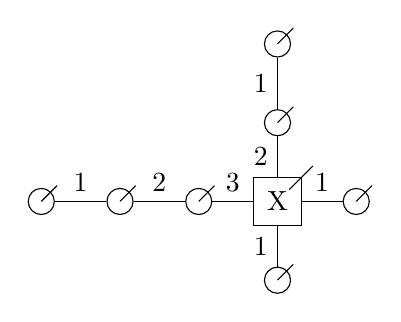
\begin{tikzpicture}[baseline=0.5]

        \def \legLength { 0.8}
        \def \radius {0.1}

        \pgfmathsetmacro{\step}{2*\radius+ \legLength} % 1
        \pgfmathsetmacro{\legpos}{\radius+\legLength} %0.9

        \node[draw,minimum size=0.6cm] (O0) at (0,0) {X};
        \draw (0.15,0.15) -- ++(0.3,0.3);

        \node[draw, circle,radius=\radius] (L1) at (-1,0) {};
        \node[draw, circle,radius=\radius] (L2) at (-2,0) {};
        \node[draw, circle,radius=\radius] (L3) at (-3,0) {};

        \node[draw, circle,radius=\radius] (U1) at (0,1) {};
        \node[draw, circle,radius=\radius] (U2) at (0,2) {};

        \node[draw, circle,radius=\radius] (D1) at (0,-1) {};

        \node[draw, circle,radius=\radius] (R1) at (1,0) {};

        \draw (O0) -- node [above] {3}  (L1);
        \draw (L2) -- node [above] {2}  (L1);
        \draw (L2) -- node [above] {1}  (L3);

        \draw (O0) -- node [left] {2}  (U1);
        \draw (U2) -- node [left] {1}  (U1);

        \draw (O0) -- node [above] {1}  (R1);

        \draw (O0) --  node [left] {1} (D1);

        \draw (L1.center) -- ++(0.2,0.2);
        \draw (L2.center) -- ++(0.2,0.2);
        \draw (L3.center) -- ++(0.2,0.2);
        \draw (U1.center) -- ++(0.2,0.2);
        \draw (U2.center) -- ++(0.2,0.2);
        \draw (R1.center) -- ++(0.2,0.2);
        \draw (D1.center) -- ++(0.2,0.2);

    \end{tikzpicture}}

\def \blockat {  \begin{tikzpicture}[baseline=0.5]

        \def \legLength { 0.8}
        \def \radius {0.1}

        \pgfmathsetmacro{\step}{2*\radius+ \legLength} % 1
        \pgfmathsetmacro{\legpos}{\radius+\legLength} %0.9

        %\node[draw=none] (O0) at (0,0) {};
        \node[draw=none,minimum size=0.6cm] (O0) at (0,0) {B};
        \draw (0.15,0.15) -- ++(0.3,0.3);

        \node[draw=none] (L1) at (-1,0) {};
        \node[draw=none] (L2) at (-2,0) {};
        \node[draw=none] (L3) at (-3,0) {};

        \node[draw=none] (U1) at (0,1) {};
        \node[draw=none] (U2) at (0,2) {};

        \node[draw=none] (D1) at (0,-1) {};

        \node[draw=none] (R1) at (1,0) {};

        %\draw (O0.center) -- ++(0.45,0.45);
        \draw (L1.center) -- ++(0.2,0.2);
        \draw (L2.center) -- ++(0.2,0.2);
        \draw (L3.center) -- ++(0.2,0.2);
        \draw (U1.center) -- ++(0.2,0.2);
        \draw (U2.center) -- ++(0.2,0.2);
        \draw (R1.center) -- ++(0.2,0.2);
        \draw (D1.center) -- ++(0.2,0.2);

        \draw (-3.3,0.3)--(-0.3,0.3) -- (-0.3,2.3)--(0.3,2.3)
        -- (0.3,0.3) -- (1.3,0.3) -- (1.3,-0.3) -- (0.3,-0.3)
        -- (0.3,-1.3) -- (-0.3, -1.3) -- (-0.3,-0.3) -- (-3.3,-0.3) -- cycle;

    \end{tikzpicture}}

\def \pepobt {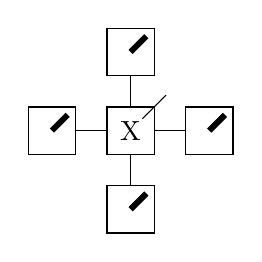
\begin{tikzpicture}[baseline=0.5]

        \def \legLength { 0.8}
        \def \radius {0.1}

        \pgfmathsetmacro{\step}{2*\radius+ \legLength} % 1
        \pgfmathsetmacro{\legpos}{\radius+\legLength} %0.9

        %\node[draw, circle, radius=\radius] (O0) at (0,0) {};
        \node[draw,minimum size=0.6cm] (O0) at (0,0) {X};
        \draw (0.15,0.15) -- ++(0.3,0.3);

        \node[draw, minimum size=0.6cm] (L1) at (-1,0) {};
        \node[draw, minimum size=0.6cm] (U1) at (0,1) {};
        \node[draw, minimum size=0.6cm] (D1) at (0,-1) {};
        \node[draw, minimum size=0.6cm] (R1) at (1,0) {};

        \draw (O0) -- (L1);
        \draw (O0) -- (U1);
        \draw (O0) -- (R1);
        \draw (O0) -- (D1);

        %\draw(O0.center) -- ++(0.2,0.2);
        \draw[line width=0.75mm]  (L1.center) -- ++(0.2,0.2);
        \draw[line width=0.75mm] (U1.center) -- ++(0.2,0.2);
        \draw[line width=0.75mm] (R1.center) -- ++(0.2,0.2);
        \draw[line width=0.75mm] (D1.center) -- ++(0.2,0.2);

    \end{tikzpicture} }

\def \blockbt {   \begin{tikzpicture}[baseline=0.5]

        \def \legLength { 0.8}
        \def \radius {0.1}

        \pgfmathsetmacro{\step}{2*\radius+ \legLength} % 1
        \pgfmathsetmacro{\legpos}{\radius+\legLength} %0.9

        %\node[draw=none] (O0) at (0,0) {};
        \node[draw=none,minimum size=0.6cm] (O0) at (0,0) {B};
        \draw (0.15,0.15) -- ++(0.3,0.3);

        \node[draw=none] (L1) at (-1,0) {};
        \node[draw=none] (L2) at (-2,0) {};
        \node[draw=none] (L3) at (-3,0) {};

        \node[draw=none] (U1) at (0,1) {};
        \node[draw=none] (U2) at (0,2) {};

        \node[draw=none] (D1) at (0,-1) {};

        \node[draw=none] (R1) at (1,0) {};

        %\draw (O0.center) -- ++(0.45,0.45);
        \draw[line width=0.75mm] (L3.center) -- ++(0.2,0.2);
        \draw[line width=0.75mm] (U2.center) -- ++(0.2,0.2);
        \draw[line width=0.75mm] (R1.center) -- ++(0.2,0.2);
        \draw[line width=0.75mm] (D1.center) -- ++(0.2,0.2);

        \draw (-3.3,0.3)--(-0.3,0.3) -- (-0.3,2.3)--(0.3,2.3)
        -- (0.3,0.3) -- (1.3,0.3) -- (1.3,-0.3) -- (0.3,-0.3)
        -- (0.3,-1.3) -- (-0.3, -1.3) -- (-0.3,-0.3) -- (-3.3,-0.3) -- cycle;

    \end{tikzpicture} }

\def \pepoct { 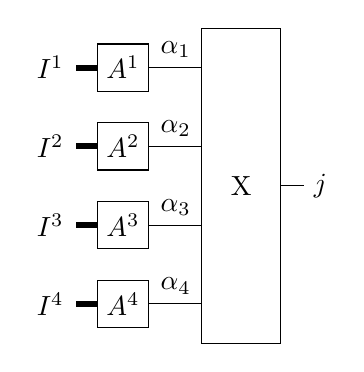
\begin{tikzpicture}[baseline=0.5]
        \draw (0,2.5)-- (0,-1.5) -- (1,-1.5)-- (1,2.5) -- cycle;

        \node[draw=none] (x)  at (0.5,0.5) {X};

        \node[draw, minimum size=0.6cm] (n1)  at (-1,2) {$A^1$};
        \node[draw, minimum size=0.6cm] (n2)  at (-1,1) {$A^2$};
        \node[draw, minimum size=0.6cm] (n3)  at (-1,0) {$A^3$};
        \node[draw, minimum size=0.6cm] (n4)  at (-1,-1) {$A^4$};

        \draw (n1) -- node [above] {$\alpha_1$} (0,2);
        \draw (n2) -- node [above] {$\alpha_2$} (0,1);
        \draw (n3) -- node [above] {$\alpha_3$} (0,0);
        \draw (n4) -- node [above] {$\alpha_4$} (0,-1);

        \draw[line width=0.75mm] (n1) -- ++(-0.6,0) node [left] {$I^1$};
        \draw[line width=0.75mm] (n2) -- ++(-0.6,0) node [left] {$I^2$};
        \draw[line width=0.75mm] (n3) -- ++(-0.6,0) node [left] {$I^3$};
        \draw[line width=0.75mm] (n4) -- ++(-0.6,0) node [left] {$I^4$};

        \draw (1,0.5) -- (1.3,0.5)  node [right] {$j$} ;

    \end{tikzpicture} }

\def \blockct { 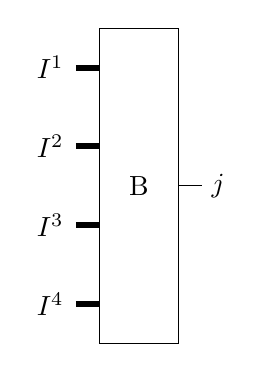
\begin{tikzpicture}[baseline=3]
        \draw (0,2.5)-- (0,-1.5) -- (1,-1.5)-- (1,2.5) -- cycle;

        \node[draw=none] (x)  at (0.5,0.5) {B};

        \draw[line width=0.75mm] (-0.3,2)  node [left] {$I^1$}  -- (0,2) ;
        \draw[line width=0.75mm] (-0.3,1)  node [left] {$I^2$} -- (0,1);
        \draw[line width=0.75mm] (-0.3,0)  node [left] {$I^3$} -- (0,0);
        \draw[line width=0.75mm] (-0.3,-1)  node [left] {$I^4$} -- (0,-1);

        \draw (1,0.5) -- (1.3,0.5)  node [right] {$j$} ;

    \end{tikzpicture} }

\noindent
An example of this procedure is
\begingroup
\allowdisplaybreaks
\begin{align}
    \pepoat                 \; & =  \;\blockat                                     \\
    \pepobt                 \; & =  \;\blockbt                                     \\
    \vcenter{\hbox{ \pepoct }} & =\vcenter{\hbox{  \blockct }} . \label{extract_x}
\end{align}
\endgroup
On the first line, the original problem is shown. Block X is the newly introduced block. The right-hand side $B$ is the residual error, i.e.\ the exponentiated Hamiltonian minus all possible contractions in the network. The second line reorders and groups the physical indices in legs, and transforms the right-hand side accordingly. The third line shows the tensors in the form of \cref{axb}, including the matching labels.

\subsubsection{Full inverse}

One way of solving this equation is by performing by contracting the grouping the matrices $A^i$ to one matrix $A = A^1 \otimes A^2 \cdots \otimes A^m$. The equation to solve is
\begin{equation}
    \begin{split}
        &A_{ I^1  I^2 \cdots I^n \alpha^1 \alpha^2 \cdots \alpha^m   } X_{ \alpha^1 \alpha^2 \cdots \alpha^m j  } \\
        = &B_{  I^1  I^2 \cdots I^m   j } .
    \end{split}
\end{equation}
The fastest way to solve this system is by using a linear solver. This results in some numerical problems. This is a result of the potentially ill conditioned inverses of legs $A^ii$, inherent to the construction. A pseudoinverse of the full matrix can be easily obtained and resolves this issue (see for numerical example \cref{subsec:inversion_procedure}). The pseudoinverse $A^{+}$ of matrix A is calculated as follows:
\begin{align}
    A     & = U \Sigma V^{\dagger}      \\
    A^{+} & = V \Sigma^{+} U^{\dagger},
\end{align}
where for $\Sigma^{+}$ all the non-zero diagonal elements are replaced by their inverse. In the numerical pseudoinverse, every singular value below a given threshold e.g.\ $\sigma_0 = 10^{-12}$ is set to zero. Linear solvers that perform a pseudoinverse also exist. The problem with this full inverse is that the bond dimension increases very fast: matrix A has dimension $d^ {2 \sum_m n_m } \cross d^ {2 \sum_m n_m } $. Although using a linear solver instead of full inversion is considerably faster, this method still becomes computationally infeasible for large systems.

\subsubsection{Sequential inverse}

A second method consist of solving the following sequence of linear problems one leg at a time
\begin{equation}
    \begin{split}
        A^1_{ I^1 \alpha^1 } X^1_{ \alpha^1  I^2 \cdots I^m j} &=  B_{  I_1  I_2 \cdots I_m   j }\\
        A^2_{ I^2 \alpha^2 } X^2_{ \alpha^1   \alpha^2  I^3 \cdots I^m j} &=  B^1_{  \alpha^1  I_2 \cdots I_m   j }\\
        &\vdots\\
        A^m_{ I^m \alpha^m } X_{ \alpha^1 \alpha^2 \cdots \alpha^m j  } &=  B^{m-1}_{ \alpha^1 \alpha^2 \cdots \alpha^{m-1} I_m   j } \;.\\
    \end{split}
\end{equation}
Here, $X^1$ is the contraction of tensor $X$ with legs $A^2$ till $A^m$. In the next step, leg $A^2$ is inverted. This continues till the last leg is inverted.
While this method is very quick and scales well, in practice it results in an unstable scheme. Solving sequentially, the errors of the pseudoinverses (or worse full inverse) accumulate. If there are 4 legs, the threshold needs to be set at $ \sigma_0 = \sqrt[4]{ 10^{-12} } $. The inverse now becomes a bad approximation of the problem, rendering the results useless (but stable).

\subsubsection{Sparse full inverse}

Luckily the problem can be resolved by first performing an \Gls{SVD} decomposition of $A^m_{ I^m \alpha^m } = U^m_{ I_m \beta^m } S^m_{\beta^m \gamma^m}  V^{m\dagger}_{\gamma^m \alpha^m}$ matrices, with S diagonal and U and V unitary. All the $U^m$ matrices can be inverted by applying the Hermitian transpose to the corresponding leg m of B. The tensor $S = S^1 \otimes S^2 \cdots \otimes S^m$ is very sparse and can be (pseudo)-inverted at once. For a full rank construction, $S$  is already diagonal. For truncated constructions (or inverses involving loops), this is no longer the case.
The last step consist of applying all the matrices $V^m$ to the right-hand side. This is shown in this equation
\begin{alignat}{1}
    A^1_{ I^1 \alpha^1 }   A^2_{ I^2 \alpha^2 }  \cdots  A^m_{ I^m \alpha^m }   X_{ \alpha^1  \alpha^2  \cdots \alpha^m j } & =  B_{  I_1  I_2 \cdots I_m   j }                 \\%%%%%%%%%%%%%%%%%%
    U^1_{ I_1 \beta^1 } S^1_{\beta^1 \gamma^1}  V^{1\dagger}_{\gamma^1 \alpha^1}                                            & \nonumber                                         \\
    U^2_{ I_2 \beta^2 } S^2_{\beta^2 \gamma^2}  V^{2\dagger}_{\gamma^2 \alpha^2}                                            & \cdots  \nonumber                                 \\
    U^m_{ I_m \beta^m } S^m_{\beta^m \gamma^m}  V^{m\dagger}_{\gamma^m \alpha^m}                                            & \nonumber                                         \\
    X_{ \alpha^1  \alpha^2  \cdots \alpha^m j }                                                                             & =  B_{  I_1  I_2 \cdots I_m   j }                 \\ %%%%%%%%%%%%%%%%%%%%%%%%%%%%%%
    S_{ (\beta^1 \beta^2 \cdots \beta^m) (\gamma^1  \gamma^2 \cdots \gamma^m)  }                                            & \nonumber                                         \\
    V^{1\dagger}_{\gamma^1 \alpha^1}   V^{2\dagger}_{\gamma^2 \alpha^2}  \cdots  V^{m\dagger}_{\gamma^m \alpha^m}           & \nonumber                                         \\
    X_{ \alpha^1  \alpha^2  \cdots \alpha^m j }                                                                             & =  B'_{  (\beta_1  \beta_2 \cdots \beta_m )  j }.
\end{alignat}
The complexity is determined by the \Gls{SVD} decomposition of the individual legs. Due to its sparsity, S does not take much space to construct and is quite fast to pseudoinvert. Doing the pseudoinverse at once means that it has the same precision as the full pseudoinverse, as desired.  It is also possible to take a pseudoinverse of a matrix with a QR-decomposition, which is faster \cite{Moylan2016}. The matrices $Q^i$ could be inverted directly, and the $R = R^1 \otimes R^2 \cdots \otimes R^m$  matrix is still upper triangular, allowing for back-substitution. This method is not used because of the memory requirements to store this matrix are larger, and the triangular matrix $R$ is not in the correct form for the linear pseudoinversion solver.

\subsubsection{Extension}
The linear solver is made for linear problems. Nevertheless, it can solve every local patch appearing in a map, such as 2 neighbouring sites. These sites are split using an \Gls{SVD} decomposition.  A problem could e.g.\ be defined as
\begin{equation}
    \vcenter{\hbox{  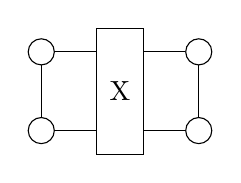
\begin{tikzpicture}[baseline=0.5]

                \def \legLength { 0.8}
                \def \radius {0.1}

                \pgfmathsetmacro{\step}{2*\radius+ \legLength} % 1
                \pgfmathsetmacro{\legpos}{\radius+\legLength} %0.9

                \node[draw, circle,radius=\radius] (L0) at (-1,0) {};
                \node[draw, circle,radius=\radius] (L1) at (-1,1) {};

                \draw (-0.3,1.3) -- (0.3,1.3) -- (0.3,-0.3) -- (-0.3,-0.3) -- cycle;

                \node[draw, circle,radius=\radius] (R0) at (1,0) {};
                \node[draw, circle,radius=\radius] (R1) at (1,1) {};

                \draw (L0) --   (L1);
                \draw (R0) --   (R1);

                \draw (L0) --   (-0.3,0);
                \draw (L1) --   (-0.3,1);

                \draw (R0) --   (0.3,0);
                \draw (R1) --   (0.3,1);

                \node[draw=none] (C0) at (0,0.5) {X};
            \end{tikzpicture} }} .
\end{equation}
The solver treats this as a linear problem with 2 legs. After that block $X$ is solved, it is decomposed as
\begin{equation}
    \vcenter{\hbox{  \begin{tikzpicture}[baseline=0.5]

                \def \legLength { 0.8}
                \def \radius {0.1}

                \pgfmathsetmacro{\step}{2*\radius+ \legLength} % 1
                \pgfmathsetmacro{\legpos}{\radius+\legLength} %0.9

                \node[draw=none, circle,radius=\radius] (L0) at (-1,0) {};
                \node[draw=none, circle,radius=\radius] (L1) at (-1,1) {};

                \draw (-0.3,1.3) -- (0.3,1.3) -- (0.3,-0.3) -- (-0.3,-0.3) -- cycle;

                \node[draw=none, circle,radius=\radius] (R0) at (1,0) {};
                \node[draw=none, circle,radius=\radius] (R1) at (1,1) {};

                \draw (L0) --   (-0.3,0);
                \draw (L1) --   (-0.3,1);

                \draw (R0) --   (0.3,0);
                \draw (R1) --   (0.3,1);

                \node[draw=none] (C0) at (0,0.5) {X};
            \end{tikzpicture} }} =  \vcenter{\hbox{  \begin{tikzpicture}[baseline=0.5]

                \def \legLength { 0.8}
                \def \radius {0.1}

                \pgfmathsetmacro{\step}{2*\radius+ \legLength} % 1
                \pgfmathsetmacro{\legpos}{\radius+\legLength} %0.9

                \node[draw=none, circle,radius=\radius] (L0) at (-1,0) {};
                \node[draw=none, circle,radius=\radius] (L1) at (-1,1) {};

                \node[draw, circle,radius=\radius] (C0) at (0,0) {};
                \node[draw, circle,radius=\radius] (C1) at (0,1) {};

                \node[draw=none, circle,radius=\radius] (R0) at (1,0) {};
                \node[draw=none, circle,radius=\radius] (R1) at (1,1) {};

                \draw (L0) --   (C0);
                \draw (L1) --   (C1);

                \draw (R0) --   (C0);
                \draw (R1) --   (C1);

                \draw (C1) --   (C0);

            \end{tikzpicture} }} .
\end{equation}
Another example is the following corner block $O^{1 \gamma \beta 0}$. It may not seem like a linear problem, but it can be solved with the linear solver without any problem
\begin{equation}
    \vcenter{\hbox{   \pepob{5}{3}{{
                        "-","-", "-",     "-",
                        "-","1","$\beta$","-",
                        "-","-","$\alpha$","-"}}{{
                        "-","-",
                        "-","-",
                        "-","$\gamma$",
                        "-","$\alpha$",
                        "-","-"}}{{
                        1,1,1,1,1,
                        1,0,0,0,1,
                        1,1,0,0,1}} }} .
\end{equation}
The algorithm will split this problem in $m=2$ legs, treating the loop as one.

\subsection{Nonlinear solver}

In some cases, the above solver does not return the best possible solution to a given problem. The reason is that it is not able to incorporate symmetries or solve problems where the new blocks appear more than once. A new solver is needed which does not rely on methods from linear algebra, but on more general nonlinear least squares solvers.

In essence, the nonlinear least squares solver needs as input a vector with the error values $\vec{f}( \vec{x} )$, and if possible also the Jacobian, i.e.\ $ J_{I,J}  = \frac{ \partial f_I }{ \partial x_J } $. This info is used to choose a direction and a step size, minimising the error. An improved point x is chosen by the algorithm, until some convergence criterium is reached. The implementation uses MATLAB's fsolve routine, which uses the Levenberg-Marquardt algorithm under the hood.

\subsubsection{Automatic differentiation}
With some care, the Jacobian can be calculated for a general \Gls{TN} in an automated way. It amounts to  contracting the network with the tensor $x_J$ removed, and treating the non-contracted indices as external ones. This becomes clearer upon inspection of \cref{extract_x}. $  \frac{ \partial B_{I^1 I^2 \cdots I^m  j } }{  \partial X_{\alpha_1 \alpha_2 \cdots \alpha_m j } } =  A_{I^1 I^2 \cdots I^m  \alpha_1 \alpha_2 \cdots \alpha_m }{}$. If a tensor appears in multiple places, the sum rule for derivatives has to be used.

% Suppose we want to differentiate the contracted tensor $T^{i_1  \cdots i_n  }$ with respect to one of the PEPO blocks $x_n = O^{i_n }_{\alpha \beta \gamma \delta}$. Denote $I=(i_1 \cdots i_n )$ and $J=(i_m  \alpha \beta \gamma \delta)$, and this block only occurs once. Then $  J_{I J}  = \frac{\partial T^{i_1  \cdots i_n  } }{  \partial O^{i_m }_{\alpha \beta \gamma \delta} } = T^{i_1 \cdots i_n } _{ i_m  \alpha \beta \gamma \delta}  \delta^{i_n}_{i_m}   $  

\subsubsection{Symmetry}

The nonlinear solver can handle rotated and permuted blocks. For instance, a simple loop (square) can be solved by rotating one tensor $O^{j }_{ \alpha \alpha 0 0}$ 4 times, once for every corner. The Jacobian is now calculated by applying the chain rule. Another example where this is useful is given in \cref{eq:rotsympepo}.

\subsubsection{Combining problems}
As only solver, the nonlinear solver can solve multiple (non-neighbouring) tensors at once, and also do this for multiple geometries at once. This does however result in slow solving times.

\subsection{Sequential linear solver}
While from the previous section it seems that all nonlinear problems need to be solved with the nonlinear solver, this is in fact not the case. This solver takes as input multiple new tensors, and solves them one by one. As this is not truly a linear system, the error will not be zero after one pass. But solving the tensors repeatedly lowers the error at each step, giving an iterative procedure. This procedure can be sped up by reusing some parts of the calculations involved in the linear solver. For example, the exponentiated Hamiltonian and contraction of all virtual levels that do not involve the optimised blocks only needs to be performed once.

The step is chosen as follows: suppose X is the current tensor and X' the newly computed one. Then the tensor is updated as follows: $X \leftarrow X + \alpha (X'-X)$. If the error has increased, the step is made smaller. The algorithm stops after a number of steps or when a certain threshold is reached.

\subsection{Conclusion}

The framework is equipped with 3 different solvers, designed to solve different problems. The code below shows how they are called from within the code:
\begin{verbatim}
[obj, ln_prefact, err] = solve_lin_and_assign(obj, map, {pattern}, 
                ln_prefact, struct);
[obj, ln_prefact, err] = solve_sequential_lin_and_assign(obj, map, {pattern},
                ln_prefact, struct, {rot_90});
[obj, ln_prefact, err] = solve_non_lin_and_assign(obj, {map}, {pattern}, 
                ln_prefact, struct, {rot_90});
\end{verbatim}
They only need a map, which is the geometry of the problem, and a pattern, i.e.\ the new block to add. \verb#rot_90# is an optional argument, listing all the permutations (such as rotation symmetry over 90 degrees). For completeness, \verb#ln_prefact# is the normalisation factor as will be discussed in the next \cref{subsec:nf}.

Whenever the linear solver can be used, it is the solver of choice. The sparse full inverse procedure is fast and handles the ill-conditioned inverses very well. The sequential linear solver builds on this solver to handle the introduction of multiple new tensors, possibly related to each other through a permutation. The nonlinear solver is at the moment only the fastest for small highly nonlinear problems, such as solving \cref{tikzfig:plaquetter} in a rotation invariant manner. The nonlinear solver can optimise multiple problems at once, and could be extended to fully use internal symmetries of the model.

\section{Optimisation}

\subsection{Bookkeeping}

One important aspect of programming these general solvers is to devise a scheme that keeps track of all the involved tensors and transforms to problem to the form described above. In the code, the geometric info is represented by a map. This keeps track of the neighbours for each site, the numeric indices of the internal and external legs and a list to perform the contractions. The solvers make only use of this info. The advantage is that for other geometries such as cyclic maps, or even other lattices, only the code to generate the maps need to be extended. These maps are used throughout the framework: to calculate the exponentiated Hamiltonians, contract the tensor networks,...

\subsection{Fast contraction}

One particular task is to determine all the possible combinations of virtual levels for a given geometry. Simply looping over all possible combinations scales as $n^m$, with n the number of virtual levels and m the number of internal legs. This quickly becomes a bottleneck.
This problem can be restated as a \Gls{PEPS} contraction in the following way: for each site make a tensor $ T^{i}_{  \alpha \beta \gamma \delta } $ where i encodes all the non-empty combinations of legs $(\alpha \beta \gamma \delta)$. On each site, the right boundary conditions need to be applied to get the right geometry. After setting the boundary conditions, the sparse \Gls{PEPS} network can be contracted and the resulting tensor gives, after decoding, all the possible contractions. Due to its sparsity, this performs quite fast.
As an added bonus, removing a tensor from T gives all contractions without this tensor. As both results are sorted, the subset of contractions containing a given tensor can also be found fast.

\subsection{Normalisation}\label{subsec:nf}

For many of the end results, the PEPO cells can be divided by a normalisation factor. Normalising the calculations is important, because $\exp( \hat{H})$ scales exponentially in the number of sites. Luckily, the exponential can be calculated directly in normalised form. Suppose H is the matrisation of the Hamiltonian evaluated for a certain geometry. This is a Hermitian matrix and can be diagonalised $H= Q D Q^{\dagger}$ with Q unitary. Then
\begin{align}
    exp(  H_{d^N} - N \alpha I  ) & =  Q exp(  D- N \log(\alpha ) I    ) Q^{\dagger} \\
                                  & =  Q \begin{bmatrix} exp(D_{1 1} - N \log(\alpha )) &        &                                     \\
                                               & \ddots &                                     \\
                                               &        & exp(D_{ d^N d^N} - N \log(\alpha )) \\
    \end{bmatrix}  Q^{\dagger}     \\
                                  & = \frac{  exp(  H_{d^N} ) }{ \alpha^N }.
\end{align}
With $I$ the unit matrix. Next to a global normalisation factor, every block calculation calculates a specific normalisation factor such that the largest eigenvalue of $exp(H)$ is of the order 1. The cut-off for pseudoinversion $\sigma_0$ is applied on the normalised problem.

\subsection{Internal representation}

Two main internal representations are used to construct the given \Gls{MPO}/ \Gls{PEPO}. Either, it is stored as a cell of tensor, one per combination of virtual levels, or as one big tensor where the blocks are added to during the construction. For sparse types, a multidimensional sparse tensor can be chosen as format. Given that MATLAB doesn't support multidimensional matrices by default, \href{https://nl.mathworks.com/matlabcentral/fileexchange/29832-n-dimensional-sparse-arrays}{this}\cite{Matt} library is used.

\subsection{Even faster inverses}

% \def \figoneb {\expH{2}{$A$}{{,}}{{,}}{{,}}}
% \def \figthreeb {\expH{3}{$B$}{{,,"$i_3$"}}{{,,"$j_3$"}}{{,"v"}}}
% \def \figtwob {\mpo{1}{{"w","v"}}{{"$i_3$",}}{{"$j_3$",}}{} {}}
% \def \figfour { \expH{1}{$A^{-1}B$}{{"$i_3$",}}{{"$j_3$",}}{{"u","v"}} }

% \begin{equation}
%     \begin{split}
%         \combineTikz{ \figoneb }{\figtwob}{1.8} &=  \figthreeb \\
%         \figtwob &= \figfour
%     \end{split}
%     \label{eq_mpoinvdef}
% \end{equation}

While the inversion procedure above states how to make use of pseudoinverses, it was not yet clear in the 1D case it was needed. The 1D implementation uses a trick to get all the inverses for free from the \Gls{SVD} decomposition. Take the \Gls{MPO} which corresponds to a unitary matrix:

% \def \figone {\expH{2}{$O^{u v,v w}$}{{"$i_1$","$i_2$"}}{{"$j_1$","$j_1$"}}{{"u","w"}}}

% \begin{equation}
%     \figone  = \mpo{2}{{"u","v","w"}}{{"$i_1$","$i_2$"}}{{"$j_1$","$j_1$"}}{}{}
% \end{equation}

% \begin{equation}
%     \begin{split}
%         U^n_{(\alpha i j) \beta} & A_{\beta \gamma} = B_{\alpha i j \gamma} \\
%         &A_{\delta \gamma} =   U^{ n\dagger}_{\delta (\alpha i j)} B_{\alpha i j \gamma}
%     \end{split}
% \end{equation}
% If we now define the \Gls{MPO} $O^{-1}_n$ equal to $U^{n \dagger}$ with the second index split and permuted:

\begin{equation}
    \mpo{1}{ {"$\alpha$","$\beta$",}  }{ { "$i$",}}{ { "$j$",}}{}{ {"$O_n$",} } \cong U^{n}_{\alpha (i j \beta)}
\end{equation}
Then the inverse \Gls{MPO} can be calculated by taking its Hermitian conjugate and reshaping.
\begin{equation}
    \mpo{1}{ {"$\beta$","$\gamma$",}  }{ { "$i$",}}{ { "$j$",}}{}{ {"$O^{-1}_n$",} } \cong U^{n \dagger}_{ (i j \beta)  \gamma }
\end{equation}
% With the notation from \cref{eq_mpoinvdef} we have:
% \def \OnBlock {\expH{4}{ $L_n^{-1} $  }{ {,,"...",} }{ {,,"...",} }{{"$\alpha$",0}} }
The inverse of the chain can be computed with a tensor contraction
\begin{equation}
    \mpo{4}{ {"$\alpha$",,,,0}  }{ {,,,,,}}{ { ,,,,,}}{{0,0,1,0}}{{"$O^{-1}_n$","$O^{-1}_m$",,"$O^{-1}_1$",} }.
\end{equation}
The physical indices need to be contracted with the corresponding indices of the tensor to apply the inverse to.

\subsection{Buffering Results}

Some calculations, such as calculating the matrix exponential, take some time. In 1D code, the same calculations were performed over and over again, and hence a buffer mechanism was written to store these results. In the 2D framework, this not necessary as the solvers only calculate the matrix exponential once and return the blocks together with the made error.

\subsection{Profiling}
To get a sense of the speed, constructing a 2D PEPO up till order 6 with level 3 truncated at bond dimension 20 with loop extensions takes about 25 seconds on my PC. The most time intensive processes involve performing the contractions. For larger systems, the time limiting factor is calculating the exponential of the Hamiltonian.

\subsection{Calculating the error}

Every solver returns the residual error for the new block. This comes at almost no cost, because all the calculations are already done during the solving procedure.

\section{Calculating phase diagrams} \label{sec:phase_diag}

This section details how the phase diagrams are calculated, stored and the critical parameters fitted. The results are discussed in \cref{subsec:2dpahsediag}.

\subsection{Points sampling}

This concerns the problem which temperatures to select to calculate the phase diagram. As  the transition between 2 phases is sharp, a uniform sampling in T is not the best option. A very fine grid is needed to capture the transition well, requiring high computation times. The sampling starts by calculating the magnetisation for N  uniformly distributed sample points between 2 temperatures. These calculations are performed in parallel on a multicore server. When they are all finished (or have run for a maximum amount of iterations), all the arch lengths are calculated, and a new T point is  repeatedly inserted in the largest interval until N new points are selected. The desired arch length $\Delta S ^2= \Delta m ^2 + r \Delta T ^2 $ between points in the m-T plane can be set, and calculations continue until the goal is reached.

\subsection{Storing the information}

Each run has a template with all the common model info. For each point 2 files are stored. One file contains the info and results, such as temperature, magnetisation, correlation length, etc. The other file is much larger and contains the PEPO tensor, the calculated \Gls{VUMPS} environments, \dots
The files of the first kind are used in other calculations, such as the fitting procedure.  Reassembling the files into one structure happens in a central function. Another function is able to reprocess already calculated points. The sampling can be continued from where it was last stopped.

\subsection{Fitting}\label{subsec:qphasediag}

The code performs a finite-size scaling as explained in \cref{subsec:fss}. The fitting procedure works as follows: a function $f_X$ defined by a limited number of parameters is made for every observable $X \in \{ m , \xi, S \}$. The parametrisation is chosen such that it has the right scaling behaviour, and the analytical derivative is known. The code performs a nonlinear optimisation, where the error is either the vertical distance to $f_X$ or the orthogonal distance. The fitted function and parameters are determined simultaneously. The optimisation runs for a limited number of cycles. Afterwards, a random displacement is made to the parameters of the current best fit. This is repeated until convergence. The code to perform this collapse was originally written by Bram Vanhecke. The adapted version includes the possibility to fit the subleading corrections and $c_i$ to calculate $\delta$.